\documentclass[12pt]{article}
\usepackage{ctex}
\usepackage[english]{babel}
\usepackage{blindtext}
\usepackage{nameref}
\usepackage{fancyhdr}
\usepackage{amsmath,amssymb,amsthm}
\usepackage{graphicx,float}
\usepackage{physics}
\usepackage{pgfplots}
\usepackage[a4paper, total={6in, 9in}]{geometry}

\graphicspath{{../image/}}

\pagestyle{fancy}
\fancyhf{}
\fancyhf[HL]{極限}
\fancyhf[CF]{\thepage}

\newcommand{\innerprod}[2]{\langle{#1},{#2}\rangle}
\newcommand{\id}{\mathtt{id}}

\newtheorem{definition}{定義}
\newtheorem*{theorem}{定理}
\newtheorem*{corollary}{衍理}
\newtheorem*{lemma}{引理}
\newtheorem*{proposition}{設理}
\newtheorem*{remark}{小記}
\newtheorem*{claim}{主張}
\newtheorem*{example}{例子}
\newtheorem*{axiom}{公設}
\renewenvironment*{proof}{\textit{證明.}}{\hfill$\qed$}

\newenvironment*{sol}{\par \textbf{解}.}{\hfill$\blacksquare$}

\begin{document}
    Reference from Introduction to Real Analysis, by R. Bartle and D. Sherbert.
    \section*{無窮小量與無窮大量}
    
    在高等數學,對於無窮的討論,一般從無窮小量開始。何爲無窮小量?即一個非常接近0的變量不斷向零靠近,而永遠無法到達0,即爲無窮小量。

    我們可以考慮數列$\{a_n\}$, 其中對於任意整數$n$,$a_n=\dfrac{1}{10^n}$。則當$n$越大時,$a_n$越靠近0。對此,記$$a_n\to 0$$考慮對任意$n$,均有$\varepsilon>0$使得$0<\varepsilon<a_n$,則稱變量$\varepsilon$為無窮小量。記$\varepsilon\to 0$。

    相對的,考慮數列$\{A_n\}$, 其中對於任意整數$n$,$A_n=10^n$。則當$n$越大時,$A_n$越靠近$\infty$。對此,記$$A_n\to \infty$$考慮對任意$n$,均有$N>0$使得$A_n<N$,則稱變量$N$為無窮大量。記$N\to \infty$。

    由此發現,無窮小量與無窮大量互相關聯:

    \begin{axiom}
        若$a_n=\dfrac{1}{A_n}$,則$$\lim_{A_n\to \infty}a_n=0$$ 
    \end{axiom}

    以上亦可簡記為$\displaystyle\lim_{x\to\infty}\frac{1}{x}=0$.

    \section*{極限的幾何概念}

    想象一個漩渦,然後有一個點$p$在漩渦裏漂浮,其結果就是\textbf{$p$會不斷沿著漩渦中心繞圈,無限接近漩渦中心,但永遠不會到達中心}。此刻,我們稱$p$所走的路綫為$p$的\textbf{軌跡},記$p(t)$並以$t>0$作時間變數,而漩渦中心$p_0$則爲$p$的軌跡的極限,記$$p_0=\lim_{t\to\infty}p(t)$$

    \begin{figure}[H]
        \centering
        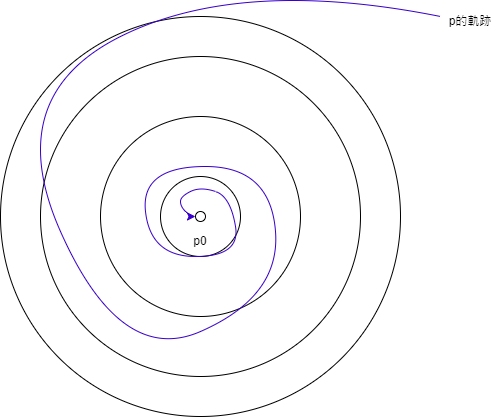
\includegraphics[scale=0.4]{limit1.png}
    \end{figure}    

    留意上圖,$p$的軌跡從外圍開始,不斷趨近於$p_0$。可見對於任何圓心為$p_0$且半徑爲$r>0$的圓形,均有$p(t)$位於圓形内。我們稱$p(t)$的極限\textbf{收斂};反之,若$p(t)$沒有唯一極限(甚至沒有極限),我們稱之爲\textbf{發散}。

    那麽,該如何證明極限收斂性成爲了微分數學一個重要命題。對此,幾何學家定名了一個數學模型,稱爲\textbf{賦距空間},指一個數學空間中,擁有計算距離的函數:

    \begin{definition}[距離函數]
        對於一個數集$S$,若函數$d:S\times S\to\mathbb{R}$符合以下條件:\begin{itemize}
            \item (正定性)對於任何$x,y\in S$,均有$d(x,y)\geq 0$;$d(x,y)=0$當且僅當$x=y$。
            \item (對稱性)對於任何$x,y\in S$,$d(x,y)=d(y,x)$。
            \item (三角不等式)對於任何$x,y,z\in S$,$d(x,z)\leq d(x,y)+d(y,z)$。
        \end{itemize}
        則稱$d$為$S$的距離函數。
    \end{definition}

    \begin{definition}[賦距空間]
        設$d$為數集$S$的距離函數,則稱$(S,d)$為賦距空間。
    \end{definition}

    \begin{example}
        若$d(x,y)=\sqrt{(x-y)^2}:\mathbb{R}\times\mathbb{R}\to \mathbb{R}$,則$(\mathbb{R},d)$為賦距空間。

        \begin{proof}
            證明函數$d$符合距離公式條件:
            \begin{enumerate}
                \item 正定性:$d(x,y)=\sqrt{(x-y)^2}\geq \sqrt{0}=0$。同時$$d(x,y)=0\iff (x-y)^2=0\iff x-y=0\iff x=y$$
                \item 對稱性:$d(x,y)=\sqrt{(x-y)^2}=\sqrt{(y-x)^2}=d(y,x)$。
                \item 三角不等式:\begin{align*}
                    [d(x,z)]^2&=(x-z)^2\\
                    &=(x-y+y-z)^2\\
                    &=(x-y)^2+2(x-y)(y-z)+(y-z)^2\\
                    &\leq [d(x,y)]^2+2[d(x,y)][d(y,z)]+[d(y,z)]^2\\
                    &=[d(x,y)+d(y,z)]^2
                \end{align*}
            \end{enumerate}
            因此,$d$為$\mathbb{R}$上的距離公式,$(\mathbb{R},d)$為賦距空間。
        \end{proof}
    \end{example}

    \begin{remark}
        此距離為絕對值函數$|\cdot|$。
    \end{remark}

    \begin{example}
        設$x=(x_1,x_2),y=(y_1,y_2)$。若$d(x,y)=\sqrt{(x_1-y_1)^2+(x_2-y_2)^2}:\mathbb{R}^2\times\mathbb{R}^2\to \mathbb{R}$,則$(\mathbb{R}^2,d)$為賦距空間。
        \begin{figure}[H]
            \centering
            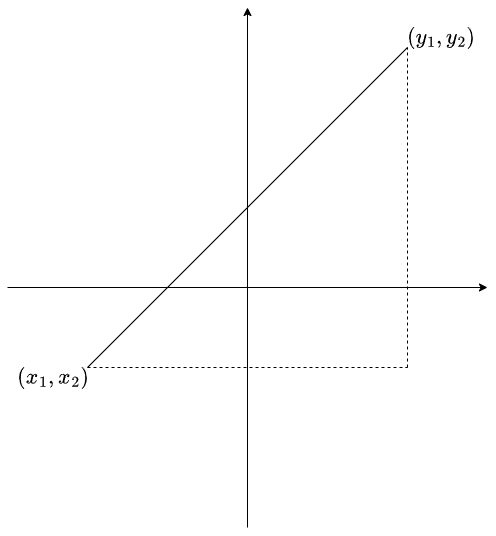
\includegraphics[scale=0.6]{EuclideanDistance.png}
            \caption{歐氏幾何:$\mathbb{R}^2=\mathbb{R}\times\mathbb{R}$即xy坐標平面}
        \end{figure}

        \begin{proof}
            證明函數$d$符合距離公式條件:
            \begin{enumerate}
                \item 正定性:$d(x,y)=\sqrt{(x_1-y_1)^2+(x_2-y_2)^2}\geq \sqrt{0}=0$。同時$$d(x,y)=0\iff (x_1-y_1)^2+(x_2-y_2)^2=0\iff \begin{cases}
                    x_1-y_1=0\\
                    x_2-y_2=0
                \end{cases}\iff x=y$$
                \item 對稱性:$d(x,y)=\sqrt{(x_1-y_1)^2+(x_2-y_2)^2}=\sqrt{(y_1-x_1)^2+(y_2-x_2)^2}=d(y,x)$。
                \item 三角不等式:證明留作習題。
            \end{enumerate}
            因此,$d$為$\mathbb{R}^2$上的距離公式,$(\mathbb{R}^2,d)$為賦距空間。
        \end{proof}
    \end{example}

    \begin{remark}
        此距離為歐式距離函數,亦稱通常距離。
    \end{remark}

    在正規數學當中,無論是在一維、二維、三維,還是更高維的賦距空間,我們都希望擁有極限收斂。利用距離公式定義收斂性,可讓我們對收斂性有更直觀的判斷。現定義於賦距空間$(S,d)$上$p$點的\textbf{$\varepsilon$-鄰域}為$$U_\varepsilon(p):=\{q\in S:d(p,q)<\varepsilon\}$$

    \begin{definition}[聚點]
        設$x(t)$為軌跡,若有$x_0$令任何$\varepsilon>0$,均有$x(t)\in U_\varepsilon(x_0)$,則$x_0$為$x(t)$的聚點。
    \end{definition}

    \begin{definition}[聚點(2)]
        設$(x_n)$為一系列點,若有$x_0$令任何$\varepsilon>0$,均有$x_n\in U_\varepsilon(x_0)$,則$x_0$為$x_n$的聚點。
    \end{definition}

    \begin{definition}[極限收斂]
        設$x_0$為$(x_n)$的聚點,而且對於任何$n>0$,均有$\varepsilon>0$使得所有$m> n$都有$x_m\in U_\varepsilon(x_0)$,則稱$x_0$為$(x_n)$的極限,或$(x_n)$收斂於$x_0$。
    \end{definition}

    \begin{example}
        設$x_n:=\dfrac{1}{n}$,則$(x_n)$在$(\mathbb{R},|\cdot|)$收斂於$0$,$\lim_{n\to \infty}x_n=0$。

        \begin{proof}
            對於任意$n>0$,均可設$\varepsilon=\frac{1}{n}$使得當$m> n$時$$d(x_m,0)=\frac{1}{m}<\frac{1}{n}=\varepsilon$$
        \end{proof}
    \end{example}

    \section*{$\varepsilon-\delta$定義-於無窮小的極限}

    當討論與函數相關時,我們必須將原有的幾何看法濃縮至代數看法,以方便計算。作爲入門理解,目前以$C(\overline{\mathbb{R}})$作討論範圍(即所有函數$f:\overline{\mathbb{R}}\to\overline{\mathbb{R}}$),這裏以$\overline{\mathbb{R}}$指代賦距空間$(\overline{\mathbb{R}},|\cdot|)$。

    $\overline{\mathbb{R}}$的定義如下:

    \begin{definition}[拓展實域]
        $\overline{\mathbb{R}}=\mathbb{R}\cup\{-\infty,+\infty\}$,同時定義:\begin{itemize}
            \item $a+\infty=+\infty+a=+\infty$,當$a\neq -\infty$;
            \item $a-\infty=-\infty+a=-\infty$,當$a\neq +\infty$;
            \item $a\cdot(\pm\infty)=\pm\infty\cdot a=\pm\infty$,當$a>0$;
            \item $a\cdot(\pm\infty)=\pm\infty\cdot a=\mp\infty$,當$a<0$;
            \item $\dfrac{a}{\pm\infty}=0$,當$a\in\mathbb{R}$;
            \item $\dfrac{\pm\infty}{a}=\pm\infty$,當$a>0$;
            \item $\dfrac{\pm\infty}{a}$,當$a<0$。
        \end{itemize}
    \end{definition}
    
    討論函數的極限,我們考慮下圖:

    \begin{figure}[H]
        \centering
        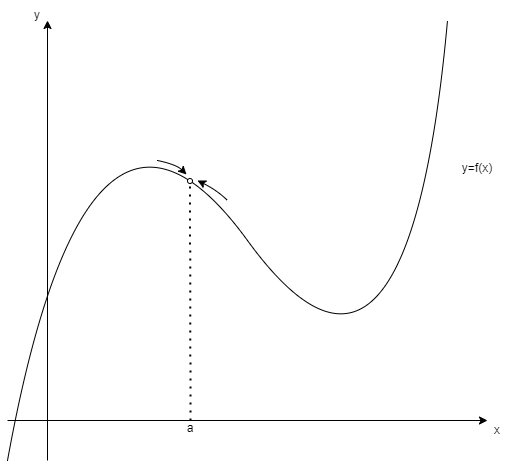
\includegraphics[scale=0.5]{function_limit.png}
    \end{figure}

    如上圖,我們希望求得$\lim_{x\to a}f(x)$的值,故以幾何角度觀看,這等同於對任意$\varepsilon>0$,當$f(x)\in U_\varepsilon(L)$時,存在$\delta>0$使得$x\in U_\delta(a)$,其中$L=\lim_{x\to a}f(x)$。

    \begin{figure}[H]
        \centering
        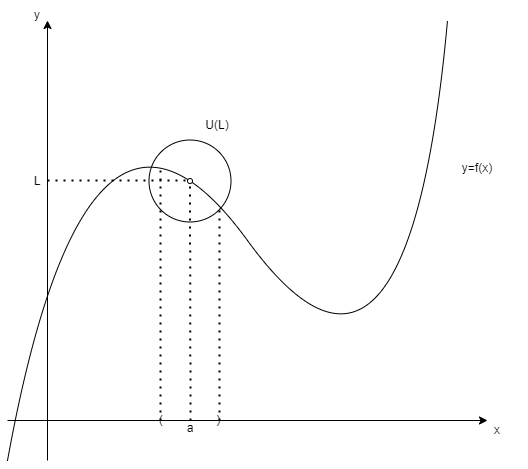
\includegraphics[scale=0.5]{epsilon-delta_limit.png}
    \end{figure}

    故此,以$|\cdot|$作爲距離函數,$x\in U_\delta(a)$等價於$|x-a|<\delta$,$y\in U_\varepsilon(L)$等價於$|y-L|<\varepsilon$,可得以下極限定理:

    \begin{theorem}
        設$f$為函數,$f$在$a$存在極限當且僅當對於任意$\varepsilon>0$,存在$\delta>0$使得所有$x$符合$0<|x-a|<\delta$時,$$|f(x)-L|<\varepsilon$$ 此則寫$L=\lim_{x\to a}f(x)$。
    \end{theorem}

    \begin{example}
        證明$\lim_{x\to a}x=a$。

        \begin{proof}
            設$\varepsilon>0$及$\delta<\varepsilon$。

            若$0<|x-a|<\delta$,則\begin{align*}
                |x-a|&<\delta\\
                &<\varepsilon
            \end{align*}
        \end{proof}
    \end{example}

    \begin{example}
        證明$\lim_{x\to a}x^n=a^n$,$n>1$為整數。
        
        \begin{proof}
            設$\varepsilon>0$及$\delta<\dfrac{\varepsilon}{nM^{n-1}}$,其中$M:=\max\{|a-\delta|,|a+\delta|\}$。

            若$0<|x-a|<\delta$,則\begin{align*}
                |x^n-a^n|&=|x-a||\sum_{i=0}^{n-1}x^ia^{n-i-1}|\\
                &\leq |x-a|\sum_{i=0}^{n-1}|x^ia^{n-i-1}|\\
                &\leq |x-a|\sum_{i=0}^{n-1}|M^iM^{n-i-1}|\\
                &=|x-a|nM^{n-1}\\
                &<\delta\cdot nM^{n-1}\\
                &<\varepsilon
            \end{align*}
        \end{proof}
    \end{example}

    從定義及定理不難發現,極限的求值無關$x=a$,説明$x=a$是一個可排除不理的點。我們稱之爲\textbf{可移去點}(point of removable discontinuity)。

    有鑒於可移去點的概念,我們求得更多難以想象、非必然但可以理解的極限的值。

    \begin{example}
        證明$\lim_{x\to a}\dfrac{x^{n+1}-a^{n+1}}{x-a}=(n+1)a^n$,$n\geq 0$為整數。
        
        \begin{proof}
            設$\varepsilon>0$及$\delta<\dfrac{2\varepsilon}{n(n+1)M^{n-1}}$,其中$M:=\max\{|a-\delta|,|a+\delta|\}$。

            若$0<|x-a|<\delta$,則\begin{align*}
                |\frac{x^{n+1}-a^{n+1}}{x-a}-(n+1)a^n|&=|\sum_{i=0}^{n}x^ia^{n-i}-(n+1)a^n|\\
                &\leq \sum_{i=0}^{n}|x^ia^{n-i}-a^n|\\
                &=\sum_{i=1}^{n}|a^{n-i}||x^i-a^i|\\
                &\leq |x-a|\sum_{i=1}^{n}|a^{n-i}|\sum_{k=0}^{i-1}|x^ka^{i-1-k}|\\
                &\leq |x-a|\sum_{i=1}^{n}M^{n-i}\sum_{k=0}^{i-1}M^kM^{i-1-k}\\
                &<\delta\cdot \sum_{i=1}^{n}iM^{n-1}\\
                &=\delta\cdot \dfrac{n(n+1)}{2}M^{n-1}\\
                &<\varepsilon
            \end{align*}
        \end{proof}
    \end{example}

    上例證得$x=a$為可移去點。

    對極限的討論,除了需要求得極限的值,還需要確定極限的唯一性,如此才能體現極限的價值。

    \begin{theorem}[唯一性]
        若$f:A\to\mathbb{R}$且$c$是$A$的聚點,則$f$在$c$點上只有一個極限。
    \end{theorem}

    \begin{proof}
        設$L,L'$均爲$\lim_{x\to c}f(x)$的值,則對於任意$\varepsilon>0$,均有:\begin{align*}
            |L-L'|&=|L-f(x)+f(x)-L'|\\
            &\leq|L-f(x)|+|L'-f(x)|\\
            &<\varepsilon/2+\varepsilon/2\\
            &=\varepsilon
        \end{align*}
    \end{proof}

    \section*{極限的性質}

    理解了極限的唯一性,現在可以更進一步探討極限的性質,包括其運算原理和重要定理。

    \begin{definition}[運算符]
        設$f,g$為實函數,則定義以下函數運算:\begin{itemize}
            \item 定義加法為$f+g$,並理解爲$(f+g)(x):=f(x)+g(x)$。
            \item 定義減法為$f-g$,並理解爲$(f-g)(x):=f(x)-g(x)$。
            \item 定義乘法為$fg$,並理解爲$(fg)(x):=f(x)g(x)$。
            \item 若$g(x)\neq 0$,定義除法為$\dfrac{f}{g}$,並理解爲$(\dfrac{f}{g})(x):=\dfrac{f(x)}{g(x)}$。
        \end{itemize}
    \end{definition}

    \begin{theorem}
        若$\lim_{x\to c}f(x)=L$及$\lim_{x\to c}g(x)=M$,則:\begin{itemize}
            \item $\lim_{x\to c}(f+g)=L+M$;
            \item $\lim_{x\to c}(f-g)=L-M$;
            \item $\lim_{x\to c}(fg)=LM$;
            \item 若$M\neq 0$,$\lim_{x\to c}(f/g)=L/M$。
        \end{itemize}
    \end{theorem}

    \begin{proof}
        加法:對於任意$\varepsilon>0$,均有:\begin{align*}
            |(f+g)-(L+M)|&=|L-f(x)+g(x)-M|\\
            &\leq|L-f(x)|+|M-g(x)|\\
            &<\varepsilon/2+\varepsilon/2\\
            &=\varepsilon
        \end{align*}
        減法:對於任意$\varepsilon>0$,均有:\begin{align*}
            |(f-g)-(L-M)|&=|f(x)-L+M-g(x)|\\
            &\leq|L-f(x)|+|M-g(x)|\\
            &<\varepsilon/2+\varepsilon/2\\
            &=\varepsilon
        \end{align*}
        乘法:對於任意$\varepsilon>0$,均有:\begin{align*}
            |(fg)-(LM)|&=|f(x)g(x)-Lg(x)+Lg(x)-LM|\\
            &\leq|g(x)||L-f(x)|+|L||M-g(x)|\\
            &<(|M|+\varepsilon)\varepsilon/(2|M|+\varepsilon)+|L|\varepsilon/2|L|\\
            &=\varepsilon
        \end{align*}
        除法:對於任意$\varepsilon>0$,均有:\begin{align*}
            |(f/g)-(L/M)|&=|Mf(x)-LM+LM-Lg(x)|/|LM|\\
            &\leq|L-f(x)|/|L|+|M-g(x)|/|M|\\
            &<|L|\varepsilon/2|L|+|M|\varepsilon/2|M|\\
            &=\varepsilon
        \end{align*}
    \end{proof}

    以上定理其實就是極限的分配律:

    \begin{itemize}
        \item $\displaystyle\lim_{x\to c}(f+g)=\lim_{x\to c}f(x)+\lim_{x\to c}g(x)$;
        \item $\displaystyle\lim_{x\to c}(f-g)=\lim_{x\to c}f(x)-\lim_{x\to c}g(x)$;
        \item $\displaystyle\lim_{x\to c}(fg)=\lim_{x\to c}f(x)\lim_{x\to c}g(x)$;
        \item 若$M\neq 0$,$\displaystyle\lim_{x\to c}(f/g)=\lim_{x\to c}f(x)/\lim_{x\to c}g(x)$。
    \end{itemize}

    \begin{proposition}
        設$f,g,h$為函數,并且對於所有$x\in\mathbb{R}$符合$g(x)\leq f(x)\leq h(x)$,若$\displaystyle \lim_{x\to c}g(x)=\lim_{x\to c}h(x)$,則$$\lim_{x\to c}g(x)=\lim_{x\to c}f(x)=\lim_{x\to c}h(x)$$
    \end{proposition}

    \begin{proof}
        設$\displaystyle \lim_{x\to c}g(x)=\lim_{x\to c}h(x)=L$,則$$-\varepsilon\leq g(x)-L\leq f(x)-L\leq h(x)-L\leq \varepsilon$$
        因此,$|f(x)-L|\leq \varepsilon$。
    \end{proof}

    以上定理汎用性極高,如下列例子:
    
    \begin{example}
        求$\lim_{n\to \infty}\dfrac{\sin{n}}{n}$。

        因$-1\leq \sin{x}\leq 1$,$$\frac{-1}{n}\leq \frac{\sin{n}}{n}\leq \frac{1}{n}\implies \lim_{n\to\infty}\frac{\sin{n}}{n}=0$$
    \end{example}
    \section*{特殊的極限}
    \begin{enumerate}
        \item $$\lim_{x\to 0}\frac{\sin{x}}{x}=1$$
        \item $$\lim_{x\to 0}\frac{e^{x}-1}{x}=1$$
    \end{enumerate}

    由於證明以上極限需使用泰勒展開式,故目前不做證明。(或以切綫解釋:需要導數基礎)
    \section*{連續函數}
    \begin{definition}[連續函數]
        設$f$為函數,$f$在$a$存在連續性當且僅當對於任意$\varepsilon>0$,存在$\delta>0$使得所有$x$符合$0<|x-a|<\delta$時,$$|f(x)-f(a)|<\varepsilon$$ 若$f$不符合以上條件,則稱$f$在$a$不連續。
    \end{definition}
    \begin{definition}
        設$f:D\to R$為函數,若$f$對所有$a\in D$均存在連續性,則稱$f$為$D$上的連續函數。
    \end{definition}
    \begin{example}
        \begin{enumerate}
            \item 常函數$f(x):=b$是$\mathbb{R}$上的連續函數。
            \item 函數$f(x):=x$是$\mathbb{R}$上的連續函數。
            \item 函數$f(x):=x^2$是$\mathbb{R}$上的連續函數。
            \item 函數$f(x):=\dfrac{1}{x}$是$\{x\in\mathbb{R}:x>0\}$上的連續函數。
            \item 函數$f(x):=\dfrac{1}{x}$不是$\mathbb{R}$上的連續函數。
            \item 函數$f(x):=\begin{cases}
                1&\textrm{若}x\textrm{為有理數}\\
                0&\textrm{若}x\textrm{為無理數}
            \end{cases}$是$\mathbb{R}$上的連續函數。
        \end{enumerate}
    \end{example}
    \begin{remark}
        若$f$不在$c$上連續,但在$c$上存在極限,則可得$$g(x):=\begin{cases}
            \lim_{x\to c}f(x) & x=c\\
            f(x) & x\neq c
        \end{cases}$$ 為連續函數。此概念多見於拓展函數。
    \end{remark}
    \section*{連續函數的性質}

    與極限相似,連續性亦擁有綫性性。

    \begin{theorem}
        若$f,g$為連續函數,則:\begin{itemize}
            \item $f\pm g, fg$均爲連續函數;
            \item 若$g\neq 0$,$f/g$為連續函數。
        \end{itemize}
    \end{theorem}

    \begin{proof}
        證明只需引用連續函數之定義即可。
    \end{proof}

    \begin{example}
        \begin{enumerate}
            \item 多項式函數:$p(x):=a_0+a_1x+a_2x^2+\cdots +a_nx^n$。
            \item 有理函數:$r(x):=\dfrac{p(x)}{q(x)}$,而$x\notin\{\alpha_i:q(\alpha_i)=0\}$。
            \item (基本)三角函數:$\sin{x}$和$\cos{x}$。

            \begin{proof}
                基於$|\sin{x}|\leq |x|$和$|\cos{x}|\leq 1$(同理,對於$\cos{x}$),可得$$|\sin{x}-\sin{c}|=2|\sin[\frac{1}{2}(x-c)]||\cos[\frac{1}{2}(x+y)]|\leq 2\cdot \frac{1}{2}|x-c|=|x-c|$$
            \end{proof}
            \item 三角函數:$\tan{x},\cot{x},\sec{x},\csc{x}$。證明從有理函數可得。
        \end{enumerate}
    \end{example}

    \begin{theorem}[複合函數的延續性]
        若$f:A\to B$, $g:C\to D$均爲連續函數,且$B\subset C$,則$$h(x):=(g\circ f)(x)=g(f(x))$$亦爲連續函數。
    \end{theorem}

    \begin{proof}
        留做習題。
    \end{proof}
    \section*{區間上的連續函數}
    
    \begin{definition}[有界性]
        函數$f:D\to R$被稱爲\textbf{在$A$上有界}若存在$M>0$使得對於任意$x\in D$,均有$|f(x)|\leq M$。
    \end{definition}

    換言之,有界性的定義在於$f$是一個值域受限的函數,以便討論極大極小值。反之,成爲無界。

    \begin{theorem}
        設$I:=[a,b]$為閉合區間,並設$f:I\to\mathbb{R}$為連續函數,則$f$在$I$上有界。
    \end{theorem}

    \begin{definition}[絕對極值]
        設$A\subset \mathbb{R}$及$f:A\to\mathbb{R}$。\begin{itemize}
            \item 若存在$x^*\in A$使得對於所有$x\in A$均有$$f(x^*)\geq f(x)$$則稱$f$有\textbf{絕對峰值},$x^*$為\textbf{峰點}。
            \item 若存在$x_*\in A$使得對於所有$x\in A$均有$$f(x_*)\leq f(x)$$則稱$f$有\textbf{絕對谷值},$x_*$為\textbf{谷點}。
        \end{itemize}
    \end{definition}
\end{document}